%!TeX root=../Dissertation.tex
%!TeX bibfile=./synthesis.bib

\chapter{System creation and setup}
\section{The host machine}
\subsection{Hardware}
It was decided as a better test of Docker's ability to reduce strain on a system, that an older machine with limited resources would be used rather than a more modern and capable machine. This was to better represent the target group of this research; that being SMEs that may have aging hardware, attempting to get the most out of what they currently have available.

The test machine has %TODO: TO DO state what the specs of the machine are. RAM, CPU, etc

\subsection{Operating System}
%TODO: To do talk about the host machines' operating system

\section{Servers}
\subsection{Operating system}
Both systems were created from scratch, using the latest LTS versions of Ubuntu Server (20.04, Focal Fossa Server \citep{UbuntuServerDocumentation}).

For VMware, the images were downloaded directly from the Ubuntu Website and the virtual machines were created using VMware's workstation Virtual Machine creation wizard, whereas for Docker, the Ubuntu Server image was taken from Ubuntu's official Docker Image, hosted on Docker Hub \citep{UbuntuDockerHub}. Each docker image was then created using a Dockerfile, which lays out which version to use; in this case, ubuntu:latest.

\subsection{Software}
\label{subsec:softwaresynth}
The servers were created to use the software and topology laid out in the requirements within section \ref{Requirements:infrastructure}.

For both VMware and Docker this meant using the Advanced Package Tool (which is the default package manager on ubuntu) to install the various software needed.

However, for VMware this was done once each server was installed and booted. On Docker, through the use of Dockerfiles, this can integrated directly into the Docker image, along with any configuration files that may be required, such as local zone files for the primary DNS server (DNS1). An example of a Dockerfile for DNS1 is shown in figure \ref{fig:dockerfileexample} below. This shows how the base image is selected, along with the addition of the software and tools necessary to make bind9 work. The `COPY' command takes the completed configuration files and places them in the correct folders.
\begin{figure}[h]
\caption{Dockerfile}
\label{fig:dockerfileexample}
\begin{minted}[frame=lines]{dockerfile}
FROM ubuntu:latest

RUN apt-get update \
  && apt-get install -y \
  bind9 \
  bind9utils \
  bind9-doc


COPY named.conf.options /etc/bind/
COPY named.conf.local /etc/bind/
COPY db.intranet.co.uk /etc/bind/
COPY db.72.168.192.in-addr.arpa /etc/bind/

CMD ["/bin/bash", "-c", "while :; do sleep 10; done"]



\end{minted}

\end{figure}

Both methods of creating the machines and grabbing software are straight forward, though I would argue that Docker, whilst maybe having a slight learning curve, is faster once the user knows that they are doing. Writing Docker files for each machine was quick and easy.

The one caveat with using Dockerfiles, however, was that during setup of phpMyAdmin on the MySQL machine, the installation process asks for user input. The Dockerfile creation process isn't intelligent enough to return these to the user so the creation of the Docker image fails in this instance. Instead, the MySQL Docker Container was created without phpMyAdmin and then once the container was created and running we could install phpMyAdmin manually. Once this is done the container in its running state must be commited to a new image using the '\texttt{docker commit}' command\citep{DockerCommit}, otherwise the changes wont be saved.

\section{Client}
\subsection{Operating System}
\label{ClientOS}
The client machine was created using VMware workstation pro, using Ubuntu's latest LTS desktop version (20.04, Focal Fossa Desktop \citep{UbuntuDesktopDocumentation})

The same client machine was used for both the VMware system and the Docker System. This was to ensure that the client used the same amount of resources (RAM, CPU and Network usage) on the host machine for both the VMware tests and the Docker tests, as in a real environment, the clients would be remote devices on the network. By using the same virtual machine as the client in both tests, any impact to the outputs of the tests should be mitigated.

The Client machine was configured to use up to 4GB of RAM, and up to two cores using VMware Workstation Pro.

\subsection{Software}
The client machine had all the testing and benchmarking software required installed before any testing took place, so that the machine was the same between testing.

The software installed was as described in the requirements list in section \ref{RequirementsListBench}. As mentioned in that section, Netdata is installed on the host machine during the final test, not the client machine. This is to ensure that usage statistics represent the whole machine, not just the client, or the endpoint (in this case, the web server).

\section{The Network}
For both tests, VMware Workstation's NAT networking mode was used \citep{VMwareNAT}. The same network was used for both in order to ensure a fair test. Using the same network provided by VMware's NAT setting ensures that any differences in network performance measured in the tests is due to factors other than the network infrastructure itself; more specifically, the difference between Docker and VMware's core performance in a network setting.

The configuration of this network was edited using VMware's "Virtual Network Settings" \citep{VMwareNetChange} to disable the built in DHCP server, so that it didn't conflict with the DHCP server created for the testing (see subsection \ref{DHCP Spec}).

Setting up VMware Virtual Machines to use the NAT (VMnet8) network is straight-forward. On the contrary, to do the Docker test, more work was required. Firstly, a Custom Docker Network named "CustomNet" was set up using Docker's "macvlan" network driver \citep{DockerMacVlan}. This network driver is designed to be bound to a physical network, similar to the "bridged" mode found in VMware, by giving each Container an individual MAC address. When creating a "macvlan" network, the interface to be used must be specified. This is where VMware's Virtual Network Adapter was used \citep{VMwareNetworkAdapter}, which is designed to allow the host machine to communicate with virtual machines over a virtualised IP interface that installed on the host machine. This allowed the Docker Network "CustomNet" to be bound to the VMnet8 interface, thus allowing the Docker containers to communicate with each other over the VMware network. This also made it possible for the VMware client to be used in the Docker test as explained in subsection \ref{ClientOS}.

Table \ref{tab:IPaddressing} shows the IP addressing and hostname scheme that was used in both tests.

\begin{table}[H]
\caption{}
\label{tab:IPaddressing}
\centering
\resizebox{\textwidth}{!}{%
\begin{tabular}{|l|l|l|}
\hline
 & \textbf{IP Address} & \textbf{DNS Hostname} \\ \hline
\textbf{DNS1} & 192.168.72.3/24 & No hostname \\ \hline
\textbf{DNS2} & 192.168.72.4/24 & ns1.intranet.co.uk \\ \hline
\textbf{DNS3} & 192.168.72.5/24 & ns2.intranet.co.uk \\ \hline
\textbf{DHCP} & 192.168.72.6/24 & dhcp.intranet.co.uk \\ \hline
\textbf{Apache} & 192.168.72.150 & www.intranet.co.uk \\ \hline
\textbf{MySQL} & 192.168.72.151 & mysql.intranet.co.uk \\ \hline
\textbf{Client Addresses} & 192.168.72.50/24 - 192.168.72.100/24 & No hostname \\ \hline
\end{tabular}%
}
\end{table}

For testing, when a server needed to be specified, the hostname was used over the IP address where applicable so that the process would make use of the DNS infrastructure. For example, 'www.intranet.co.uk' is used in the Jmeter test, instead of '192.168.72.150'.

\subsection{Difficulties with Docker and DHCP}
\label{Difficulties with Docker and DHCP}
As mentioned above, Docker was using the 'macvlan' Docker network driver. This network driver is not the recommended driver for use by Docker, as generally Containers in Docker are designed to run within the constraints of the machine they are running on, and not to face out onto a physical network. Due to this, there was an occasion during the creation of the Docker system whereby the DHCP server was not giving our IP addresses even though it was configured to do so.

After trying various troubleshooting methods, and after rebooting several times, it seemed there was no solution to the problem. It was decided that we would come back to the issue the following day with a fresh mind. After booting up Docker fresh the following day, the DHCP server started working as intended. I believe the issue was due to the way the Docker handles replies over IP, as it seemed to be dropping important packets headed into the DHCP container that were part of the DHCP handshake process (The process would restart from the beginning again, and then the returning packets would drop in a continuous loop). This is however, merely hypothesis, as if I had the real solution to the problem I was facing I would certainly explain it in more detail, but this erroneous behaviour was never observed again. 

Even after the Docker containers were saved to .tar files, and then reloaded onto different hardware, the DHCP server ran entirely as expected. I would suggest this speaks to the fact that this work is on the edge of what Docker is really designed to do, so your own tests and observations on your own hardware, may in-fact differ.



%Talk about which install is easier, and things that might be worth mentioning about how these two are managed and what that means for those that might want to use these services.



\chapter{Testing \& Benchmarks}
Introductory explanations for each of these tests and benchmarks are included in the requirements in section \ref{RequirementsListBench}.

\section{Test 1 - iPerf3 Throughput}
\label{sec:Test1}
\subsection{Test parameters}
In this test, the throughput is measured between the Apache server and the Client. The listener for iPerf3 was setup on the Apache server using port 5201 (the default port for iPerf3 \citep{iPerf3Documentation}). The client then specifies that is is in-fact running iPerf3 as a client, and tells the server which format to record throughput with. For this testing, the format used was 'M', meaning Megabytes \citep{iPerf3Documentation}.

The test runs for ten seconds, taking measurements of total throughput in a second, resulting in ten points that can be converted into a graph showing the transfer rate (throughput) over time in Megabytes per second. An average can also be taken from this. A separate throughput is calculated on each side of the transaction (at the server, and at the client).
 
\subsection{Results}
\label{test1results}
The average throughputs for both tests, and for clients and severs, are shown in table \ref{tab:iperf3average} below.

\begin{table}[h]
\centering
\caption{Table showing the average transfer rate in a 10 second period}
\label{tab:iperf3average}
\resizebox{\textwidth}{!}{%
\begin{tabular}{|c|c|c|}
\hline
x & \textbf{VMware Average (MBytes/s)} & \textbf{Docker Average (MBytes/s)} \\ \hline
\textbf{Client} & 176.37 & 290.70 \\ \hline
\textbf{Apache Server} & 172.61 & 290.40 \\ \hline
\end{tabular}%
}
\end{table}

The averages shown in this table clearly show a higher throughput for the Docker system, with an improvement (averaged between the Client and the Apache Server) of 116.06 MegaBytes per Second.

Figure \ref{fig:test1graphs} shows the transfer rate over time for both Client and Server.

\begin{figure}[H]
\caption{}
\label{fig:test1graphs}
\fbox{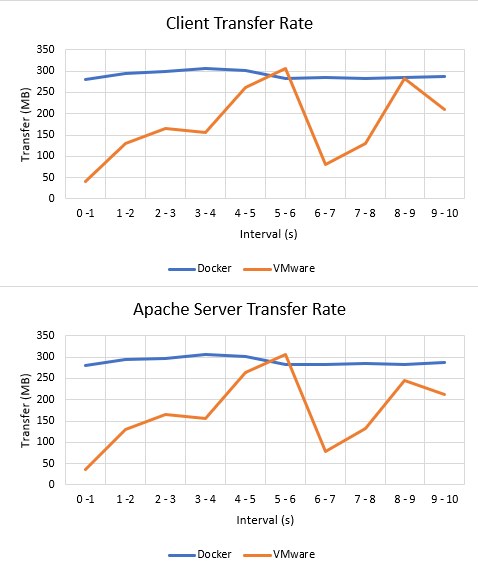
\includegraphics[width=0.8\textwidth]{./synthesis/test1graphs.PNG}}
\centering
\end{figure}

This shows that Docker is stable, whilst VMware's throughput result fluctuates far more. This would suggest that the VMware system is unstable; something we will investigate further in the evaluation section of this report.

\section{Test 2 - Sysbench MySQL Input/Output}
\label{sec:Test2}
\subsection{Test parameters}
This test required a test database with random data to be created on the MySQL server. Luckily, Sysbench includes a 'prepare' tool, which allows a user to specify parameters of for the table that match the test they want to conduct \citep{sysbench}. Sysbench then creates, or \emph{prepares}, a database that is suitable for said test. A test user account with all permissions was also created for Sysbench to use. When the prepare command is run, it creates the database and tables, and then fills the tables with the amount ant type of data specified.

The database we created for testing had the following parameters:
\begin{itemize}
  \item The database had two tables.
  \item Each table had a size of 500000.
  \item Table size in sysbench relates to rows. Meaning across the two tables, there was a total of one million rows of data.
  \item The test was specified as '\texttt{oltp\_read\_write}'.
\end{itemize}

OLTP is Online Transaction Processing\citep{oltpbenchmarking}, which is a term used to describe online databases that generally have high throughput and connectivity from many users \citep{oracleoltp}. The \texttt{oltp\_read\_write} test attempts to simulate an OLTP workload by performing various different SELECT, DELETE, INSERT and UPDATE queries on the data \citep{sysbenchmarking}.

Once the above table was created, the actual test could be performed. The client machine runs the command that starts the test, and the domain name for the MySQL server (mysql.intranet.co.uk) was used to specify where the server and database were located.

The test was run using the following parameters:
\begin{itemize}
  \item The port was set as 3306 (the default for MySQL).
  \item Two threads were used. This simulates the database being accessed and changed by two different users or programs at the same time.
  \item 'Time' was set as 300. This is in seconds, meaning the scenario ran for five minutes.
  \item 'Events' was set as 0. This setting would allow the user to specify that the test should stop after a certain number of events have been reached. By setting this to '0', the test will continue to run until the 'Time' setting is reached.
\end{itemize}
\subsection{Results}
\label{test2results}

Figure \ref{fig:test2fiveminutes} shows the total number of Read, Write and Other queries performed by Sysbench in a 5 minute period. The results for both systems are compared side by side.

This graph shows a clear win for Docker, with the VMware system managing to perform just over a third of the number of Reads that Docker managed in the same time frame.

\begin{figure}[H]
\caption{}
\label{fig:test2fiveminutes}
\fbox{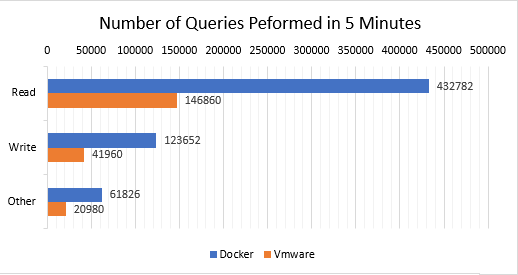
\includegraphics[width=\textwidth]{./synthesis/test2fivemingraph.png}}
\centering
\end{figure}

Figure \ref{fig:test2onesecgraph} shows both the total queries per second, and the total transactions per second for both systems. A query is defined as being a single statement such as SELECT, INSERT or UPDATE\citep{mysqlqueries}; whereas a transaction is a combination of multiple of these statements within one command\citep{mysqltransactions}, typically in order to manipulate multiple rows of data.

This further shows just how much faster the Docker system was at data manipulation.

\begin{figure}[H]
\caption{}
\label{fig:test2onesecgraph}
\fbox{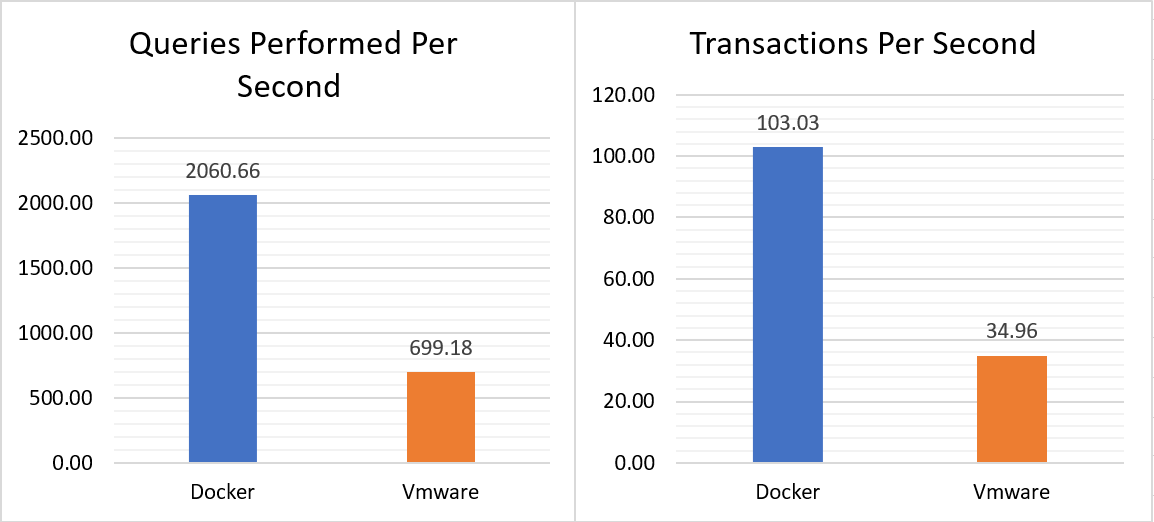
\includegraphics[width=\textwidth]{./synthesis/test2onesecgraph.PNG}}
\centering
\end{figure}

The latency between queries was also measured by Sysbench. Figure \ref{test2latencygraph} shows a latency bar graph, with the minimum, average, and 95th percentile latencies in Milliseconds. The 95th percentile was rather than the maximum, because both tests experienced a maximum latency that would have dwarfed the other results. These maximum latencies were also most likely errors (which were to be expected with such a high number of queries being performed \citep{oltpbenchmarking}).

\begin{figure}[H]
\caption{}
\label{test2latencygraph}
\fbox{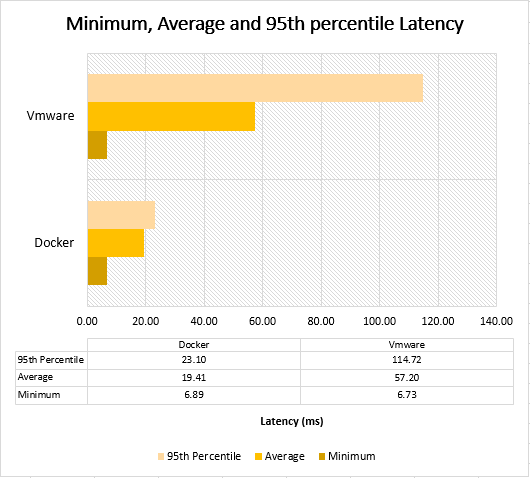
\includegraphics[width=0.90\textwidth]{./synthesis/test2latencygraph.PNG}}
\centering
\end{figure}

We can see from these results, that Docker far out performs VMware in terms of latency, to such an extreme extent that Dockers' top 95th percentile results are lower than VMware's average latency.

\section{Test 3 - Namebench}
\label{sec:Test3}
\subsection{Test parameters}
This test compares the performance of the DNS servers and their ability to perform DNS queries for various websites.

Namebench works by going through a list (specified by the user) of websites and recording the latency for the DNS server to perform the query\citep{Namebench}. Before the test commenced, the caches on all of the DNS servers in our infrastructure were wiped to ensure a fair test between the two systems. In our testing, the following parameters were set:
\begin{itemize}
  \item The list to be used was specified as 'alexa'. This option uses Amazon's Alexa Top Sites list \citep{alexainternet}. Around 38,000 different website addresses were tested. Having a high number of tests is important because it gives a good average.
  \item Both DNS2 and DNS3 were specified (using their domain names: ns1.intranet.co.uk and ns2.intranet.co.uk respectively) to be tested. DNS1 is a primary server, and is hidden in the network topology, only to be used as the master for the 'intranet.co.uk' domain, so it isn't tested here.
\end{itemize}

\subsection{Results}
Figure \ref{fig:test3graphaverage} shows a graph of the average DNS response times. We can see from this graph that Docker has smaller average DNS response when compared to VMware. An interesting, but unrelated behaviour here is that DNS2 in both tests out performed DNS3; this is unexpected given that both servers share exactly the same configuration. Perhaps this is a characteristic of the way that BIND9 handles secondary DNS servers?

\begin{figure}[H]
\caption{}
\label{fig:test3graphaverage}
\fbox{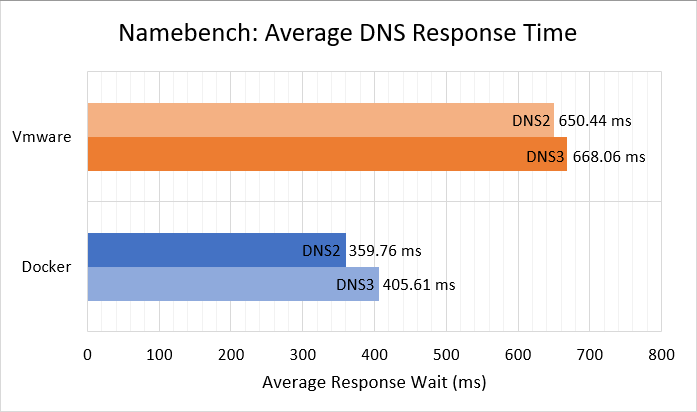
\includegraphics[width=0.8\textwidth]{./synthesis/test3graphaverage.PNG}}
\centering
\end{figure}

We can see the minimum latency response in figure \ref{fig:test3graphmin}. Here, Docker takes the win again, with a similar relative margin between results as with the average latency shown above. Here we can see that the latency for each server is the same within the same system; this helps us to rule out an element of chance to the results (ie, the results are more likely to be genuine given that they are the same across the two severs for the same system).

\begin{figure}[H]
\caption{}
\label{fig:test3graphmin}
\fbox{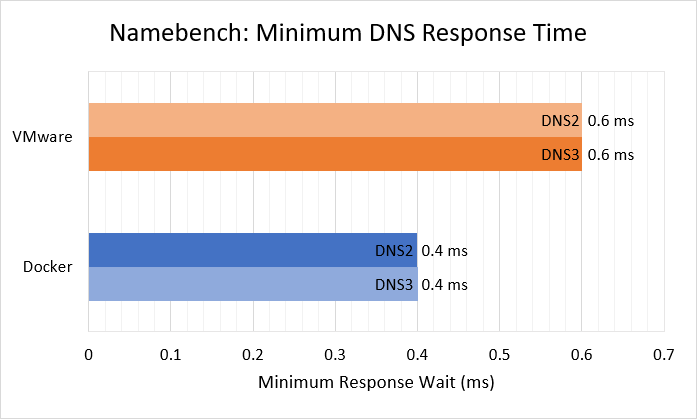
\includegraphics[width=0.8\textwidth]{./synthesis/test3graphmin.PNG}}
\centering
\end{figure}

No maximum latency is given in a graph as in both tests, certain requests hit their maximum wait time for a response (3500ms). This is most likely due to an error with authoritative servers outside of our control. Furthermore, 95th percentile data could not be used (such as in our last test in subsection \ref{test2results}) because Namebench compiles the the minimum, average and maximum data itself, without allowing the user to access raw data. (Most likely because the domain name list provided by Alexa \citep{alexainternet} is propriety, so providing access to this data could be a breach of Alexa's agreements.

\section{Test 4 - Apache JMeter and Performance measurements using Netdata}
\label{sec:Test4}
\subsection{Test parameters}
\label{Test4TestParameters}
%the idle benchmarks didn't have the client machine running!
This test is slightly different, in that the data we get back from the workload (JMeter) isn't the most important piece of data we receive by doing the test. Instead, we are using the workload that is generated using JMeter \citep{ApacheJMeter}, in order to measure the stress on the machine (though we do still look at the data JMeter found). The three areas of Computing performance we will be looking into here are the CPU usage, RAM usage and the 'Load' on the machine. These were measured using Netdata\citep{Netdata}, so that the data could be monitored on another PC without affecting the performance of the PC running the Containers and Virtual Machines. Netdata also creates real-time graphs that can can then be saved in snapshots, so that we can investigate the results in depth.

Idle data was also collected from Netdata. In these idle tests, the whole system was live, but without the client machine running. When the test with the JMeter load was done, the whole system, \emph{including} the client was active. The reason for taking idle data, was so that we have a baseline figure to compare to for when the system was under stress.

JMeter was used to test the Apache server, and the JMeter tool was installed and run from the client (the same as the other tests). JMeter works by the user creating a test plan\citep{JMeter3}, in which a number of different parameters can be set to create a test workload that is exactly what the user requires. The below parameters were specified for JMeter:
\begin{itemize}
  \item A new thread group was created. A thread group is essentially a group of simulated users, with each individual 'thread' being one user \citep[3.1 Thread Group]{JMeter3}, that to Apache, will appear as a different client. This is what allows JMeter to do stress testing.
  \item Within this thread group, we set the number of 'threads' to 100. The ramp-up period was also set as 100. The ramp up period is the amount of time (in seconds) that Jmeter takes to start all threads\citep[3.1 Thread Group]{JMeter3}. The time between starting one thread and starting the next is equal to \(\frac{Time(s)}{ThreadCount}\) \citep[3.1 Thread Group]{JMeter3}. In this case, \(\frac{100}{100}=1\). So the time between each thread start is one second. The loop count within this thread group was set to 10, this means each thread (user) will perform the test 10 times before that thread closes.
  \item Now that we have our thread group, we need to assign it a task. This is done by adding both a 'sampler' and a 'configuration' element. A sampler allows us to do various requests\citep[3.2.1 Samplers]{JMeter3} but in this case we will be doing a HTTP request. The configuration element, allows us to change the options within the sampler \citep[3.6 Configuration Elements]{JMeter3}. For our test we used the 'http request defaults' config element; the only change we make is to set the domain to \texttt{www.intranet.co.uk}.
  \item Finally, we need to add a listener. A listener is a way to collect the results that are generated by JMeter\citep[3.3 Listeners]{JMeter3}. As we wanted to be able to compile the results ourselves, we used the 'view results in table' listener\citep[18.3 Listeners, View Results in Table]{JMeter18}, which allows us to export the results to a CSV file for easy data manipulation later.
\end{itemize}

\subsection{Results}
\subsubsection{JMeter}
Table \ref{tab:Test4Average} shows the average latency for both the Docker System and the VMware system. We can see that Docker has a reduced average when compared to VMware; further strengthening support for the Docker system.

\begin{table}[H]
\centering
\caption{}
\label{tab:Test4Average}
\resizebox{0.5\textwidth}{!}{%
\begin{tabular}{|c|c|}
\hline
\multicolumn{2}{|c|}{AVERAGE   LATENCY (ms)} \\ \hline
Docker                & Vmware               \\ \hline
5.85                  & 8.88                 \\ \hline
\end{tabular}%
}
\end{table}

The parameters we set gave us an output that had the latency for 1000 HTTP request transactions. To better illustrate the spread of latency, Figure \ref{fig:Test4JMeterGraph} shows the frequency of these latencies. Frequency relates to the number of times a certain latency (in ms) was recorded. A latency of 0ms means the system took less than 1ms to process the HTTP request. Some latencies have been grouped together as they became less frequent.

\begin{figure}[H]
\caption{}
\label{fig:Test4JMeterGraph}
\fbox{\includegraphics[width=\textwidth]{./synthesis/Test4JMeterGraph.PNG}}
\centering
\end{figure}

Firstly, we can see that Docker had far more response times in the 0ms category. This suggests the Docker system often didn't have a backlog of requests due to be being saturated meaning it was still able to give almost instant replies. Moving to the next category, we can see that both Docker and VMware have similar numbers of requests in the 1ms range, however, Docker is still slightly ahead. Moving on to the 2ms range, we can see than VMware starts to take over as having more counts of this latency. Moving past this latency we can see that VMware has far more responses in the higher latency ranges, with 36 counts in \(9ms+\) range, compared to only \(7\) counts for Docker.

If we dig deeper into these \(9+\) results, we can see that some of them are incredibly high in comparison to what we would expect. For Docker, of the seven results in the \(9+\) category, five of them are in in the magnitude of \(10^1ms\). One of the results in in the magnitude of \(10^2ms\) but is also the first result in the series, so can be omitted as a `warmup' result. The one other result here is \(4635ms\), which clearly shows an erroneous result.

To look at VMware's 36 results in the 9+ category it is easier to break it down into table \ref{tab:vmwareJMeterAnom}.

\begin{table}[H]
\centering
\caption{Magnitude of latencies for VMware that are over \(9ms\)}
\label{tab:vmwareJMeterAnom}
\resizebox{0.6\textwidth}{!}{%
\begin{tabular}{|l|l|}
\hline
\textbf{Latency Magnitude} & \textbf{Count} \\ \hline
\(10^1\)       & 28             \\ \hline
\(10^2\)       & 6              \\ \hline
\(10^3\)      & 2              \\ \hline
\end{tabular}%
}
\end{table}

From this table, we can see that six results took between \(100ms\) and \(999ms\)(One of these is also the first result, so should be considered a `warmup' result, as have done the same with Docker. A further two results take \(1036ms\) and \(3996ms\). When compared with Docker, this demonstrates how these anomalous results or `hitches' in the system were more common in VMware.

\subsubsection{Netdata}
\textbf{CPU Usage:}
First, we will look at idle CPU usage. Important to remember, in subsection \ref{Test4TestParameters} we discussed that the idle usages were taken without the client running. This means that the idle usages are reflective of the usage we would see in a live environment on this hardware, if the system was receiving no traffic.

Figure \ref{fig:DockerCPUIdle} shows Docker's CPU usage at idle
\begin{figure}[H]
\caption{Docker Idle CPU}
\label{fig:DockerCPUIdle}
\fbox{\includegraphics[width=\textwidth]{./synthesis/Test4dcpuidle.PNG}}
\centering
\end{figure}


Figure\ref{fig:VMwareCPUIdle} shows VMware's CPU usage at idle.
\begin{figure}[H]
\caption{VMware Idle CPU}
\label{fig:VMwareCPUIdle}
\fbox{\includegraphics[width=\textwidth]{./synthesis/Test4vmcpuidle.PNG}}
\centering
\end{figure}

Already we can see that VMware is using far more resources from the CPU when idle compared to Docker.
Figure \ref{fig:DockerCPUwork} shows the CPU usage of the Docker system for when the JMeter test was being performed.
\begin{figure}[H]
\caption{Docker JMeter Workload CPU}
\label{fig:DockerCPUwork}
\fbox{\includegraphics[width=\textwidth]{./synthesis/Test4dcpuwork.PNG}}
\centering
\end{figure}

Figure \ref{fig:VMwareCPUwork} shows the CPU usage of the VMware system whilst under stress from the JMeter test.
\begin{figure}[H]
\caption{VMware JMeter Workload CPU}
\label{fig:VMwareCPUwork}
\fbox{\includegraphics[width=\textwidth]{./synthesis/Test4vmcpuwork.PNG}}
\centering
\end{figure}

Whilst the difference during a workload is less noticeable, it is still clear that VMware's CPU usage is more than Dockers. Interestingly, we can see that the Docker's usage ramps up at the start of the test, but begins to drop once the test has been running for some time. This might suggest that Docker manages consistent workloads more efficiently.

\textbf{RAM Usage:}
Here we will investigate the RAM usage on the system. To start, Figure \ref{fig:DockerRAMidle} shows the machine's RAM usage whilst running the Docker system idle. We can see from this, that when idle, the docker system takes up very little RAM on the host machine

\begin{figure}[H]
\caption{Docker Idle RAM}
\label{fig:DockerRAMidle}
\fbox{\includegraphics[width=\textwidth]{./synthesis/Test4dramidle.PNG}}
\centering
\end{figure}

Figure \ref{fig:VMwareRAMidle} shows the RAM usage on the host machine when the VMware system is running in idle. We can see that there is a very tiny amount of free RAM, which could be a considerable bottleneck to the system, or cause it thrash \citep{thrashing}. However, the portion of RAM actively being 'used' is also fairly small (still more than the Docker system, but not unreasonable). Instead most of the RAM is is cached. This is most probably due to the way that VMware partitions away sections of RAM for its virtual machines. The ram we see cached is most likely being used to host each individual virtual machine .

\begin{figure}[H]
\caption{VMware Idle RAM}
\label{fig:VMwareRAMidle}
\fbox{\includegraphics[width=\textwidth]{./synthesis/Test4vmramidle.PNG}}
\centering
\end{figure}

Moving onto Docker under a load from the JMeter test (Figure \ref{fig:DockerRAMwork}), we see that there is a slight increase in 'used' RAM, and considerably more ram being cached. There is still a healthy amount of RAM left free for the system to use, so no thrashing should take place.

\begin{figure}[H]
\caption{Docker JMeter Workload RAM}
\label{fig:DockerRAMwork}
\fbox{\includegraphics[width=\textwidth]{./synthesis/Test4dramwork.PNG}}
\centering
\end{figure}

Figure \ref{fig:VMwareRAMwork} shows the RAM for the host machine whilst under a workload from the JMeter test. There is very little change between the usage here and the usage at idle (Figure {fig:VMwareRAMidle}), other than the RAM buffers being slightly reduced. This is because even at idle, the system is already fully committed; there is no free ram for the machine to move into. This might explain why some of our previous results for VMware, such as in subsection \ref{test1results} (Test 1 Results), are unstable.

\begin{figure}[H]
\caption{VMware JMeter Workload RAM}
\label{fig:VMwareRAMwork}
\fbox{\includegraphics[width=\textwidth]{./synthesis/Test4vmramwork.PNG}}
\centering
\end{figure}

\textbf{Load:}
Whilst CPU and RAM usage are self explanatory, 'load' may seem more vague. Load as measured by Netdata, is defined in the same way that Ferrari et al. defines load, whereby load is based on the number of tasks using the CPU and I/O along with those that are waiting in a queue\citep{loadferrari}. This is as opposed just using CPU utilisation on its own, as this combined approach gives better results as to the actual extended load of the system. By measuring load in this way, we are also tying in other parts of the hardware, as load could increase with little CPU utilisation, if for example the machine was waiting for memory resources to be clear. Netadata access this data by using linux's built in "\texttt{/proc/loadavg}" file \citep{systemload}.

By looking at load in this way, we effectively tie the two measurements above (CPU and RAM) with other hardware (for example; the disk) to see what the combined affect is to the machine.

Figure \ref{fig:Dockerloadidle} shows the Netdata load graph for Docker whilst idle. In this graph, 'load1', 'load5' and 'load15' refer to the number of of tasks waiting on over one, five and fifteen minute averages respectively. Generally low results across the board is best, however, we can see in this graph that 'load1' has a few spikes, however the scale of this graph is actually designed to show load at all times. If we look at the y axis, we can see that the axis is actually showing 0.70 as the highest number, which relatively speaking means less than one task a second is taking 5 minutes in the queue.

\begin{figure}[H]
\caption{Docker Idle Load}
\label{fig:Dockerloadidle}
\fbox{\includegraphics[width=\textwidth]{./synthesis/Test4dloadidle.PNG}}
\centering
\end{figure}

Figure \ref{fig:VMwareloadidle} shows the idle load for VMware. Here, we can see just how much of an affect on task completion times having multiple virtual machines running has on the system. Again, notice the y axis goes much higher here, and that there are more tasks waiting 15 minutes, than there are 5 or 1. Around three and a half tasks are waiting more than fifteen minutes to be processed.

\begin{figure}[H]
\caption{VMware Idle Load}
\label{fig:VMwareloadidle}
\fbox{\includegraphics[width=\textwidth]{./synthesis/Test4vmloadidle.PNG}}
\centering
\end{figure}

Figure \ref{fig:Dockerloadwork} shows the Load on the host machine when docker was under stress from the JMeter test. We can see from the Y axis that around two tasks are waiting more than a minute to be completed at peak. There is around one task at worst waiting 15 minutes.

\begin{figure}[H]
\caption{Docker Workload Load}
\label{fig:Dockerloadwork}
\fbox{\includegraphics[width=\textwidth]{./synthesis/Test4dloadwork.PNG}}
\centering
\end{figure}

Figure \ref{fig:VMwareloadwork} displays the Load during the same JMeter test, but on the VMware system. We can see here that more tasks are taking longer than 15 minutes than otherwise. Looking at the y axis, we can also see that the bars are sitting far higher than the previous graphs. Interestingly, we can see that load is on a downwards slope even during a workload. So whilst load here may be very high, we could maybe hypothesise that should the load continue long enough, that the machine may reach some sort of equilibrium.

\begin{figure}[H]
\caption{VMware Workload Load}
\label{fig:VMwareloadwork}
\fbox{\includegraphics[width=\textwidth]{./synthesis/Test4vmloadwork.PNG}}
\centering
\end{figure}
0